
The DESY-type beam telescope are tabletop tracking detectors featuring six pixelated silicon sensors, four scintillators with photo multiplier tubes (PMTs) for trigger purposes,
 a Trigger Logic Unit (TLU) providing trigger logic and time stamp information on particle passage, and a data acquisition system for the data readout. 
Figure\,\ref{fig:datura-tscope} shows the beam telescope with its sensor jigs, wherein the pixel sensors are embedded, with its auxiliary boards providing connections for power,
 sensor configuration, clock signals, and data transmission. 
The planes are organised in two telescope arms holding three sensors each. 
A DUT can be inserted between the arms or at either end of the beam telescope. 
In the Cartesian, right-handed coordinate system chosen, the $x$-direction points horizontally and $z$-direction along the beam.

\begin{figure}[tb]
	\center
	\includegraphics[width=.9\textwidth]{figures/DATURA.jpg}
	\caption[The $\Datura$ telescope]{The $\Datura$ beam telescope with its sensor planes on aluminium rails.
	The auxiliary boards with connections for clock signals, sensor configuration, and data lines are mounted at the top of the jigs.
	Coolant is provided to the jigs via the tubes.}
	\label{fig:datura-tscope}
\end{figure}
 
\subsection{Sensors and mechanics}
\label{sec:sensors}

The $\Mimosa$ detectors used for precise spacial measurement of particle trajectories are manufactured with the 350\,nm CMOS technology. 
Each $\Mimosa$ detector consists of pixels sized $\unit{18.4}{\upmu\meter} \times \unit{18.4}{\upmu\meter}$, which are arranged in 1152 columns and 576 rows.
This adds to a total of about four million readout channels covering an active area of about $\unit{10.6}{\milli\meter} \times \unit{21.1}{\milli\meter}$. 
The $\Mimosa$ sensors have been thinned down to $\unit{50}{\upmu\meter}$ and are protected on each side by $\unit{25}{\upmu\meter}$ lightproof Kapton foil. 
Free charge carriers produced in the underlying \unit{14}{\upmu\meter} epitaxial layer are mainly collected via diffusion. 
The binary resolution of $\unit{5.3}{\upmu\meter}$ can be improved by charge sharing, as will be shown in section~\ref{sec:trackres}.
%With the rising industrial interest in high resistivity epitaxial silicon for CMOS detectors the production cost of improved noise and radiation hardness parameters
% became already possible with ~400 Ohm·cm for 10 μm epitaxial layer for $\Mimosa$. 

The $\Mimosa$ sensors are read out with a rolling-shutter, taking 16\,cycles of an 80\,MHz clock per row, with all columns being read out in parallel. 
This allows for correlated double sampling and zero suppression on-chip with the digital circuitry placed outside the active pixel array. 
At this clock frequency, the $\Mimosa$ integration time equals $\unit{115.2}{\upmu\second}$ and allowing for about 8680 frames to be read out per second. 
The expected maximum rate of detectable particles through the active area estimates to be about $\unit{1}{\mega\hertz/\centi\meter^2}$ due to the limited on-chip buffer size. 
The detection threshold is programmable via so-called JTAG files. 
These provide configurations with different threshold levels in integer multiples $\noise$ of the RMS noise of the individual planes. 
A sensor threshold setting of six therefore corresponds to a collected charge in a single pixel of at least six times the noise. 
The average noise occupancy per read-out frame is measured to be smaller than $2\cdot10^{-5}$ at room temperature and a signal-to-noise threshold of six.

Every pixel sensor is mounted within an aluminium jig, three jigs are in turn mounted on each of the two aluminium arms. 
The jigs feature a beam window around the position of the sensor location, minimising the material budget. 
The overall material of the beam telescope thus amounts to $\unit{300}{\upmu\meter}$ of silicon and $\unit{300}{\upmu\meter}$ of Kapton. 
The two telescope arms, usually one up- and one downstream of the DUT, is movable along the direction of the beam in order to allow for variably sized DUTs to be fitted into the set-up. 
The minimal distance between two sensors is given by the jig thickness of 20\,mm, the maximal distance is restricted by the length of the aluminium arms to 150\,mm at equidistant spacing.
Furthermore, the jigs are cooled keeping the $\Mimosa$ sensors at a constant temperature allowing for stable operation.
The entire beam telescope is placed on a rotatable frame easing adjustment of its orientation parallel to the beam. 
Additionally, this frame is mounted on a sturdy structure providing stability over time and wheels for easy transportation. 

Important parameters are compiled in figure~\ref{fig:datura_sketch}. 
The distance between $\Mimosa$ planes is denoted as $\dz$, the distance between the DUT and its nearest neighbouring $\Mimosa$ planes $\dzdut$. 
The expression $\epsilon = \sum_i x_{i}/X_{0,i}$ defines the material budget of the scattering medium as the material thickness normalised to its radiation lengths,
 with values of $X_0 = 93.65\,\milli\meter$ for silicon, $X_0 = 3.042\cdot 10^{5}\,\milli\meter$ for dry air, and $X_0 = 285.6\,\milli\meter$ for Kapton.\,\cite{ref:x0values}
The material budget of a $\Mimosa$ plane including a protecting Kapton foil on each side is $\epsmimo = 7.1\cdot10^{-4}$. 
Likewise, the DUT's material budget is called $\epsdut$ and includes the DUT itself and other material such as PCBs and cooling boxes.


\begin{figure}[tb]
	\center
	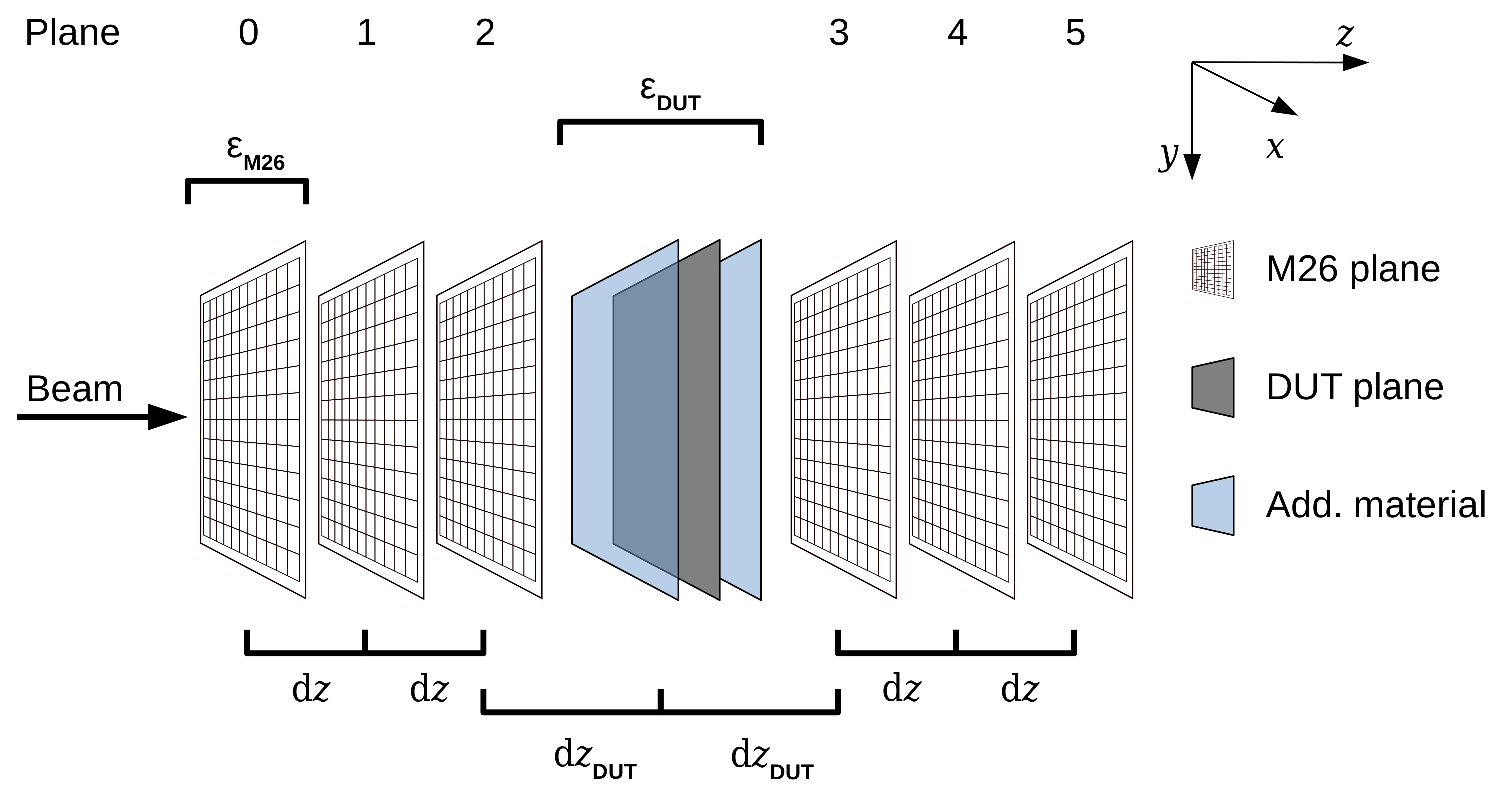
\includegraphics[width=.9\textwidth]{figures/sketch_tscope4}
	\caption[Sketch of the DESY-type telescope set-up]{Sketch of the DESY-type telescope set-up and its important parameters.}
	\label{fig:datura_sketch}
\end{figure}

\subsection{Trigger and DAQ system}

Four Hamamatsu PMTs assemblies with scintillators and lightguides, two in front and two in the back of the telescope, define the spatial acceptance window for triggers. 
The crossed scintillators on either side of the beam telescope define a rectangular acceptance window of $10\,\milli\meter \times 20\,\milli\meter$ matching the $\Mimosa$ acceptance area. 
The TLU, based on a commercial Spartan\,3 board, features a coincidence unit with discriminator boards accepting up to four PMT inputs signals. 
Additionally, it is equipped with several custom-made add-on PCBs allowing for an easy integration of user DAQ systems. 
Providing a programmable logic, the TLU  takes a trigger decision and distributes the trigger signal to all DAQ systems.
As interface to the beam telescope DAQ and other DUTs, the TLU provides RJ45 connectors with four LVDS pairs carrying the trigger clock, the busy line, the reset line, and a trigger line. 
The data clock and the busy line are inputs to the TLU, whereas the reset and the trigger line are outputs. In addition, a LEMO interface is available providing trigger output and inputs for the busy and reset signals.

The TLU accepts a busy signal from each integrated device individually halting the issue of the next trigger if the busy signal is high. 
The handling of the trigger/busy signals can be done in three handshake modes, one being the ``no-handshake'' mode,
 in which the TLU issues a fixed-length pulse on the trigger line with the busy line being disregarded. 
In simple handshake mode, the assertion of a trigger is replied by the DUTs by asserting a signal on the busy line. 
The TLU then de-asserts the trigger, and waits for busy going low on the busy line in order to be able to issue a subsequent trigger.
The normal handshake uses the same scheme as in the simple trigger mode, but additionally trigger data is transferred on the trigger line:
After the trigger has been de-asserted, the trigger number is clocked out via this line using the rising edges of the trigger clock as clock enable for the shift register holding the trigger data. 
The reset line is used to signal the reset of the timestamp counter.

The $\Mimosa$ sensors provide zero-suppressed hit data over a flat ribbon cable to the auxiliary boards, which provide RJ45 connectors to connect them with the
 data concentrator board collecting the data from all six sensors and the trigger/busy lines from the TLU. 
A 52-pin cable then transports the data and the TLU trigger/busy lines in parallel into a FlexRIO board, which is equipped with analogue-to-digital converters and an FPGA. 
The $\Mimosa$ data from the rolling-shutter readout is written continuously to RAM without taking into account the trigger information. 
The data is then available via direct memory access to the DAQ software framework and an event is written to disk in normal handshake mode, only if a trigger has been raised for a certain telescope readout frame. 

